\section{On the first category of the tangent lines on two circles}

Here, the purpose is to determine both the exact contact point of the tangents of the two circle and the intersection point of those tangent lines.

\begin{proposition}
Let $(C_1)$ and $(C_2)$ two circles such as given in the following figure. Therefore :
\begin{equation}
\gamma = \frac{\pi}{2} - \arcsin{\frac{r_1 - r_2}{d}}
\end{equation}
\end{proposition} 

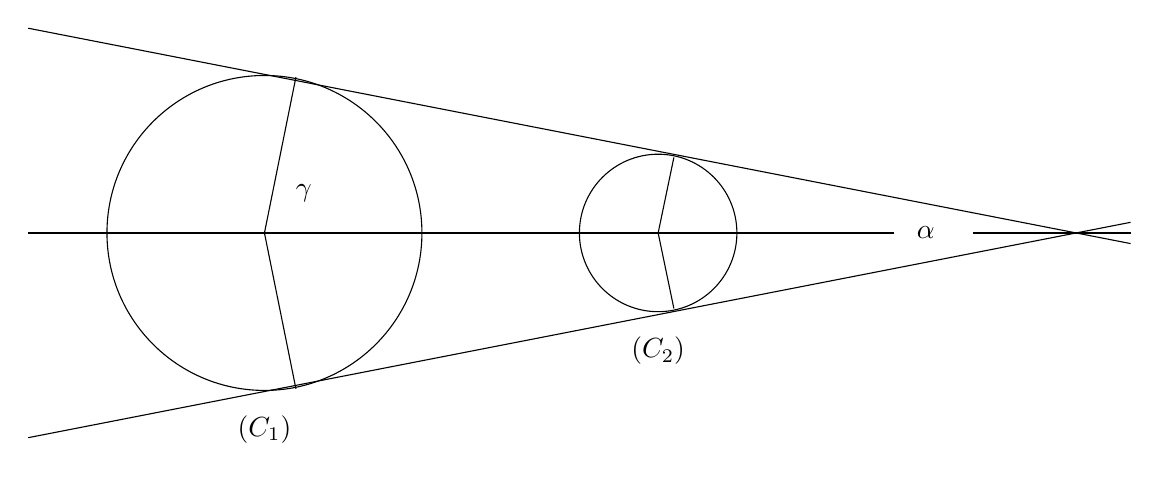
\begin{tikzpicture}

\tkzDefPoints{0/0/A, 0.4/1.98/B, 5/0/C, 5.2/0.96/D}

\draw (0,0) circle (2);


\draw (5,0) circle (1);

\draw (-3,-2.6) -- (11,0.135);
\draw (-3,2.6) -- (11,-0.135);

\draw (0, 0) -- (0.4, 1.98);
\draw (0, 0) -- (0.4, -1.98);

\draw (5, 0) -- (5.2, 0.96);
\draw (5, 0) -- (5.2, -0.96);

\draw (-3, 0) -- (8, 0);
\draw (9,0) -- (11,0);

\tkzMarkAngle[size=0.6](B, A, C)

\node at (0,-2.5) {$(C_1)$};
\node at (5,-1.5) {$(C_2)$};
\node at (0.5, 0.5) {$\gamma$};
\node at (8.4,0) {$\alpha$};



\end{tikzpicture}
